\documentclass{csc_assignment4}
\usepackage[utf8]{inputenc}
\usepackage[letterpaper, portrait, margin=1in]{geometry}
\usepackage{calc}  % arithmetic in length parameters
\usepackage{enumitem}  % more control over list formatting
\usepackage{fancyhdr}  % simpler headers and footers
\usepackage{lastpage}  % for last page number
\usepackage{relsize}  % easier font size changes
\usepackage[normalem]{ulem}  % smarter underlining
\usepackage{url}  % verb-like typesetting of URLs
\usepackage{xfrac}  % nicer looking simple fractions for text and math
\usepackage{amsmath}
\usepackage{amssymb}
\usepackage{tikz}
\usepackage{algorithm}
\usepackage{algorithmic}
\usepackage{graphicx}
\usepackage{listings}
\graphicspath{{/}}
\usepackage[export]{adjustbox}
\usepackage{enumitem}
\usepackage{subcaption}
\usepackage{esvect}

 \lstset{breaklines=true}

% ----------------------------------------------------------------
% TODO: Enter the assignment number, your name, and your student number below
% ----------------------------------------------------------------
\AssignmentName{Assignment 3}
\StudentName{Akhil Gupta}
\StudentNumber{1000357071}

% ----------------------------------------------------------------
\begin{document}
\begin{description}

\item[Q1.]
\begin{enumerate}[label=(\alph*)]
\item
\begin{lstlisting}[language=MATLAB]
% read image
im = imread('data/door.jpg');

imshow(im);
disp('click on the four corners of the luggage. Double click the last point');
[x,y] = getpts();
close all;
imshow(im);

% dimensions of luggage in px
x2 = [1, 175, 175, 1]';
y2 = [1, 1, 280, 280]';

% compute homography
tform = maketform('projective',[x,y],[x2,y2]);
[imrec] = imtransform(im, tform, 'bicubic','XYScale',1);

% get height and width
imshow(imrec);
disp('Click on the length of the door. Double click the second point');
[x_height, y_height] = getpts();
disp('Click on the width of the door. Double click the second point');
[x_width, y_width] = getpts();

height = sqrt((x_height(1) - x_height(2))^2 + (y_height(1) - y_height(2))^2)/100;
width = sqrt((x_width(1) - x_width(2))^2 + (y_width(1) - y_width(2))^2)/100;

disp (height); % in cms
disp (width); % in cms

>> door_script
click on the four corners of the luggage. Double click the last point
Click on the length of the door. Double click the second point
Click on the width of the door. Double click the second point
   60.9856 

   200.7282 

\end{lstlisting}
\begin{figure}[h]
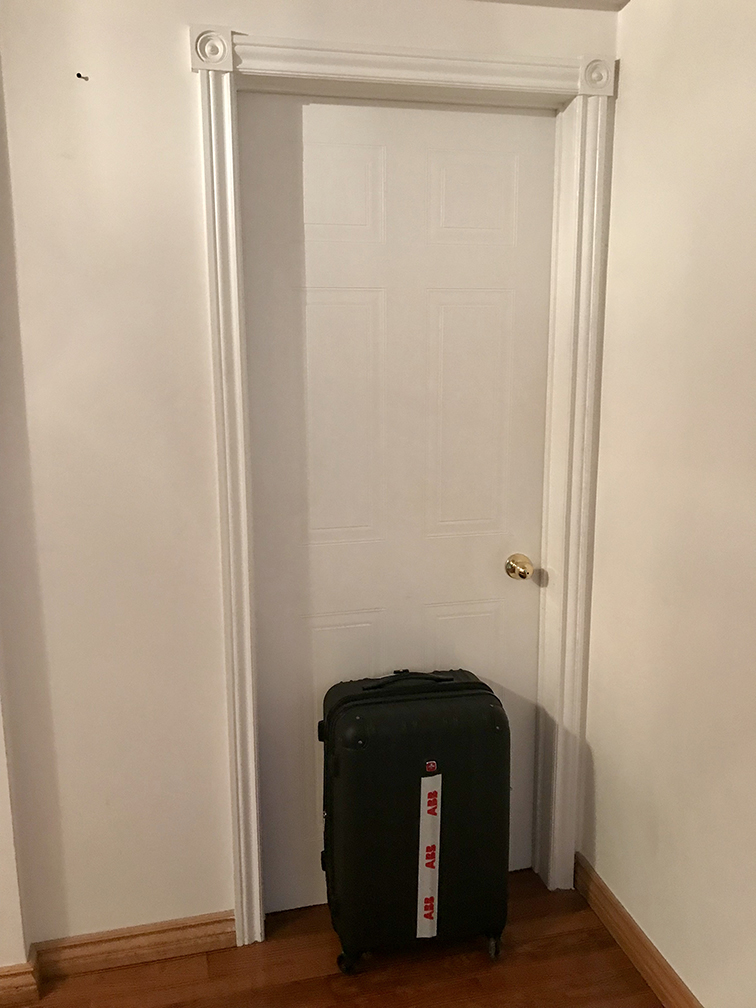
\includegraphics[width=0.6\textwidth, center]{data/door.jpg}
\vspace*{-5mm}
\caption{Luggage to scale outside my door}
\end{figure}
\begin{figure}[h]
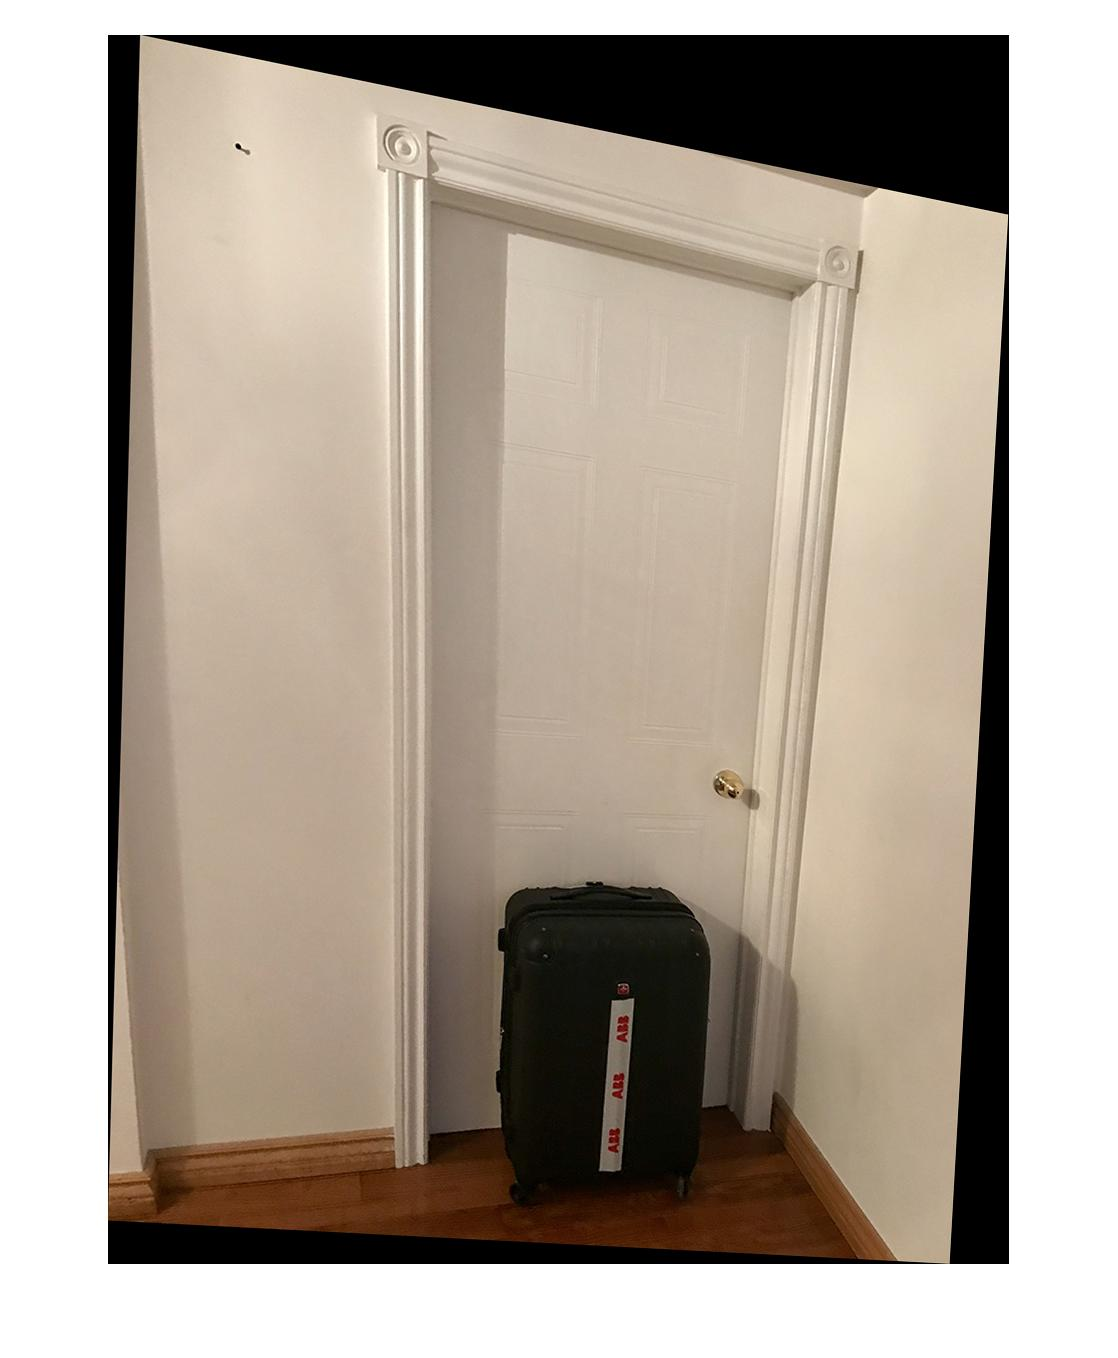
\includegraphics[width=0.6\textwidth, center]{data/trans_door.jpg}
\vspace*{-15mm}
\caption{Output after computing homography}
\end{figure}

\newpage
\item[Q2.] Stitch 2 Images:
\begin{lstlisting}[language=Python]
import cv2
import numpy as np

# Read input images
img1 = cv2.imread('data/landscape_1.jpg')
img2 = cv2.imread('data/landscape_2.jpg')

# Use SIFT to find keypoints and compute homography matrix
M =  compute_sift(img1, img2)

# Stitch the images together using homography matrix
result_image = stitch_images(img2, img1, M)

# Show stitched image
cv2.imshow ('Stitched Image', result_image)
cv2.waitKey()


def compute_sift(img1, img2):
	# Initialize SIFT 
	sift = cv2.xfeatures2d.SIFT_create()

	# Extract keypoints and descriptors
	k1, d1 = sift.detectAndCompute(img1, None)
	k2, d2 = sift.detectAndCompute(img2, None)

	# Bruteforce matcher to be run on descriptors
	bf = cv2.BFMatcher()
	matches = bf.knnMatch(d1,d2, k=2)

	threshold = 0.8
	final_matches = []
	for m1, m2 in matches:
		if m1.distance < threshold * m2.distance:
			final_matches.append(m1)

	min_matches = 8
	if len(final_matches) > min_matches:
		img1_pts = []
		img2_pts = []

		for match in final_matches:
			img1_pts.append(k1[match.queryIdx].pt)
			img2_pts.append(k2[match.trainIdx].pt)

		img1_pts = np.float32(img1_pts).reshape(-1,1,2)
		img2_pts = np.float32(img2_pts).reshape(-1,1,2)
		
		# Compute homography
		M, mask = cv2.findHomography(img1_pts, img2_pts, cv2.RANSAC, 5.0)
		return M

def stitch_images(img1, img2, M):
	# get size of input images
	w1, h1 = img1.shape[:2]
	w2, h2 = img2.shape[:2]

	img1_dims = np.float32([ [0,0], [0,w1], [h1, w1], [h1,0] ]).reshape(-1,1,2)
	img2_dims_temp = np.float32([ [0,0], [0,w2], [h2, w2], [h2,0] ]).reshape(-1,1,2)

	# Get perspective of second image
	img2_dims = cv2.perspectiveTransform(img2_dims_temp, M)

	result_dims = np.concatenate((img1_dims, img2_dims), axis = 0)

	# Calculate dimensions of match points
	[x_min, y_min] = np.int32(result_dims.min(axis=0).ravel() - 0.5)
	[x_max, y_max] = np.int32(result_dims.max(axis=0).ravel() + 0.5)
	
	# Create output array after affine transformation 
	transform_dist = [-x_min,-y_min]
	transform_array = np.array([[1, 0, transform_dist[0]], [0, 1, transform_dist[1]], [0,0,1]]) 

	# Warp images
	result_img = cv2.warpPerspective(img2, transform_array.dot(M), (x_max-x_min, y_max-y_min))
	result_img[transform_dist[1]:w1+transform_dist[1], transform_dist[0]:h1+transform_dist[0]] = img1

	return result_img
	
***  OUTPUT ON NEXT FEW PAGES  ***
\end{lstlisting}


\begin{figure}[h!]
  \centering
  \begin{subfigure}[b]{0.5\linewidth}
    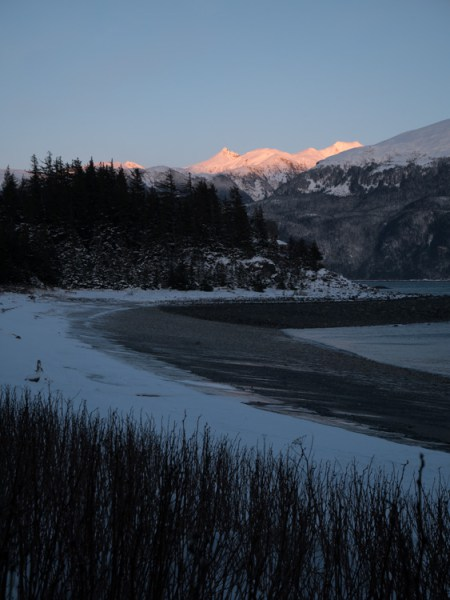
\includegraphics[width=\linewidth]{data/landscape_1.jpg}
    \caption{landscape 1.jpg provided to us}
  \end{subfigure}
  \begin{subfigure}[b]{0.5\linewidth}
    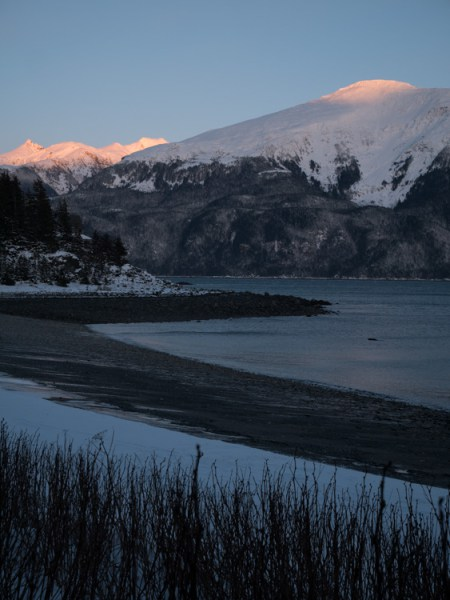
\includegraphics[width=\linewidth]{data/landscape_2.jpg}
    \caption{landscape 2.jpg provided to us}
  \end{subfigure}
\end{figure}

\clearpage
\begin{figure}[t!]
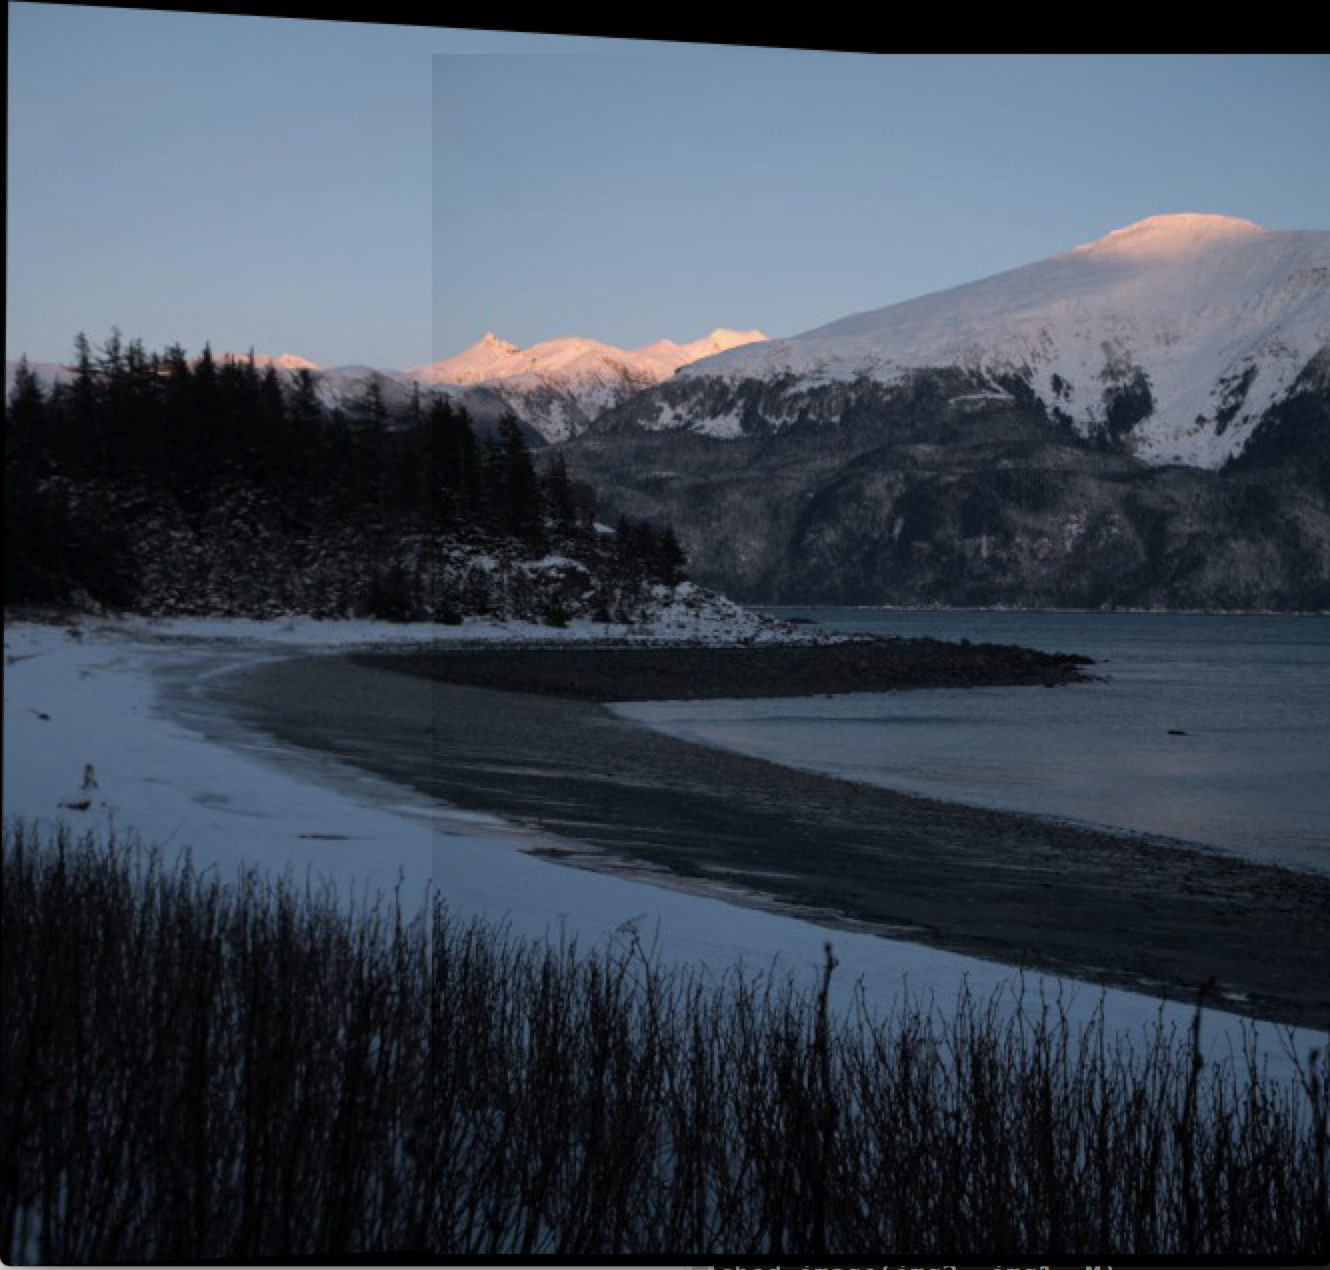
\includegraphics[width=0.7\textwidth, center]{stitched_image_2.png}
\caption{Stitched 2 images to create mini-panorama}
\end{figure}

\item[Q3.]
\begin{lstlisting}[language=MATLAB]
K =  [[725,    0, 620.5],
      [  0,  725, 187.0],
      [  0,    0,     1]];
  
baseline = 1.0;

img = imread('data/rgb.png');
disparity = double(imread('data/disparity.png'))/256;

Z = (725*baseline)./(disparity);

i = 1;
for r = 1:size(Z, 1)
    for c = 1:size(Z, 2)
        xyz(i, :) = (K \ [c-1 ; r-1; 1])' * Z(r,c);
        i = i + 1;
    end
end

X = xyz(:,1);
Y = xyz(:,2);
Z = xyz(:,3);

surf(xyz, img, 'FaceColor', 'texturemap', 'EdgeColor', 'none')
view(0, 1200)
axis manual

*** OUTPUT ON THE NEXT PAGE ***
\end{lstlisting}

\begin{figure}[h!]
  \centering
  \begin{subfigure}[b]{0.8\linewidth}
    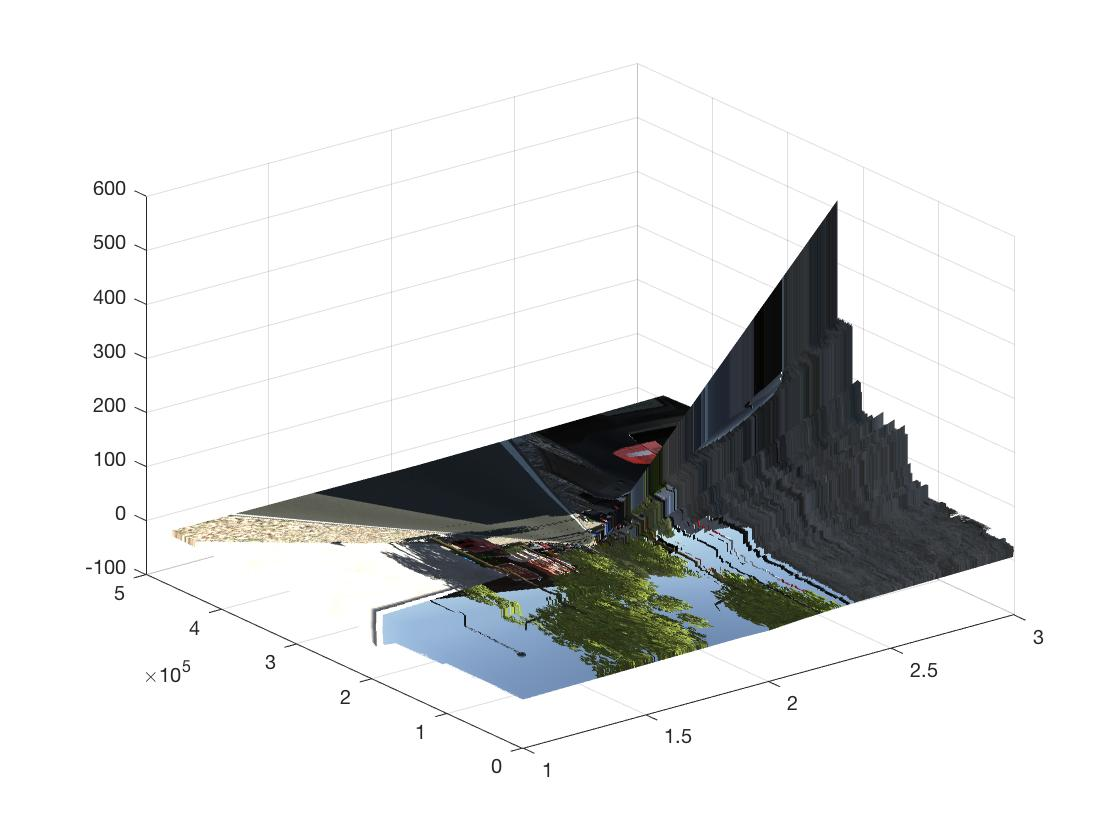
\includegraphics[width=\linewidth]{rgb-d.jpg}
    \caption{Output 3D scene (approved by Professor via Piazza Post @76)}
  \end{subfigure}
  \begin{subfigure}[b]{0.8\linewidth}
    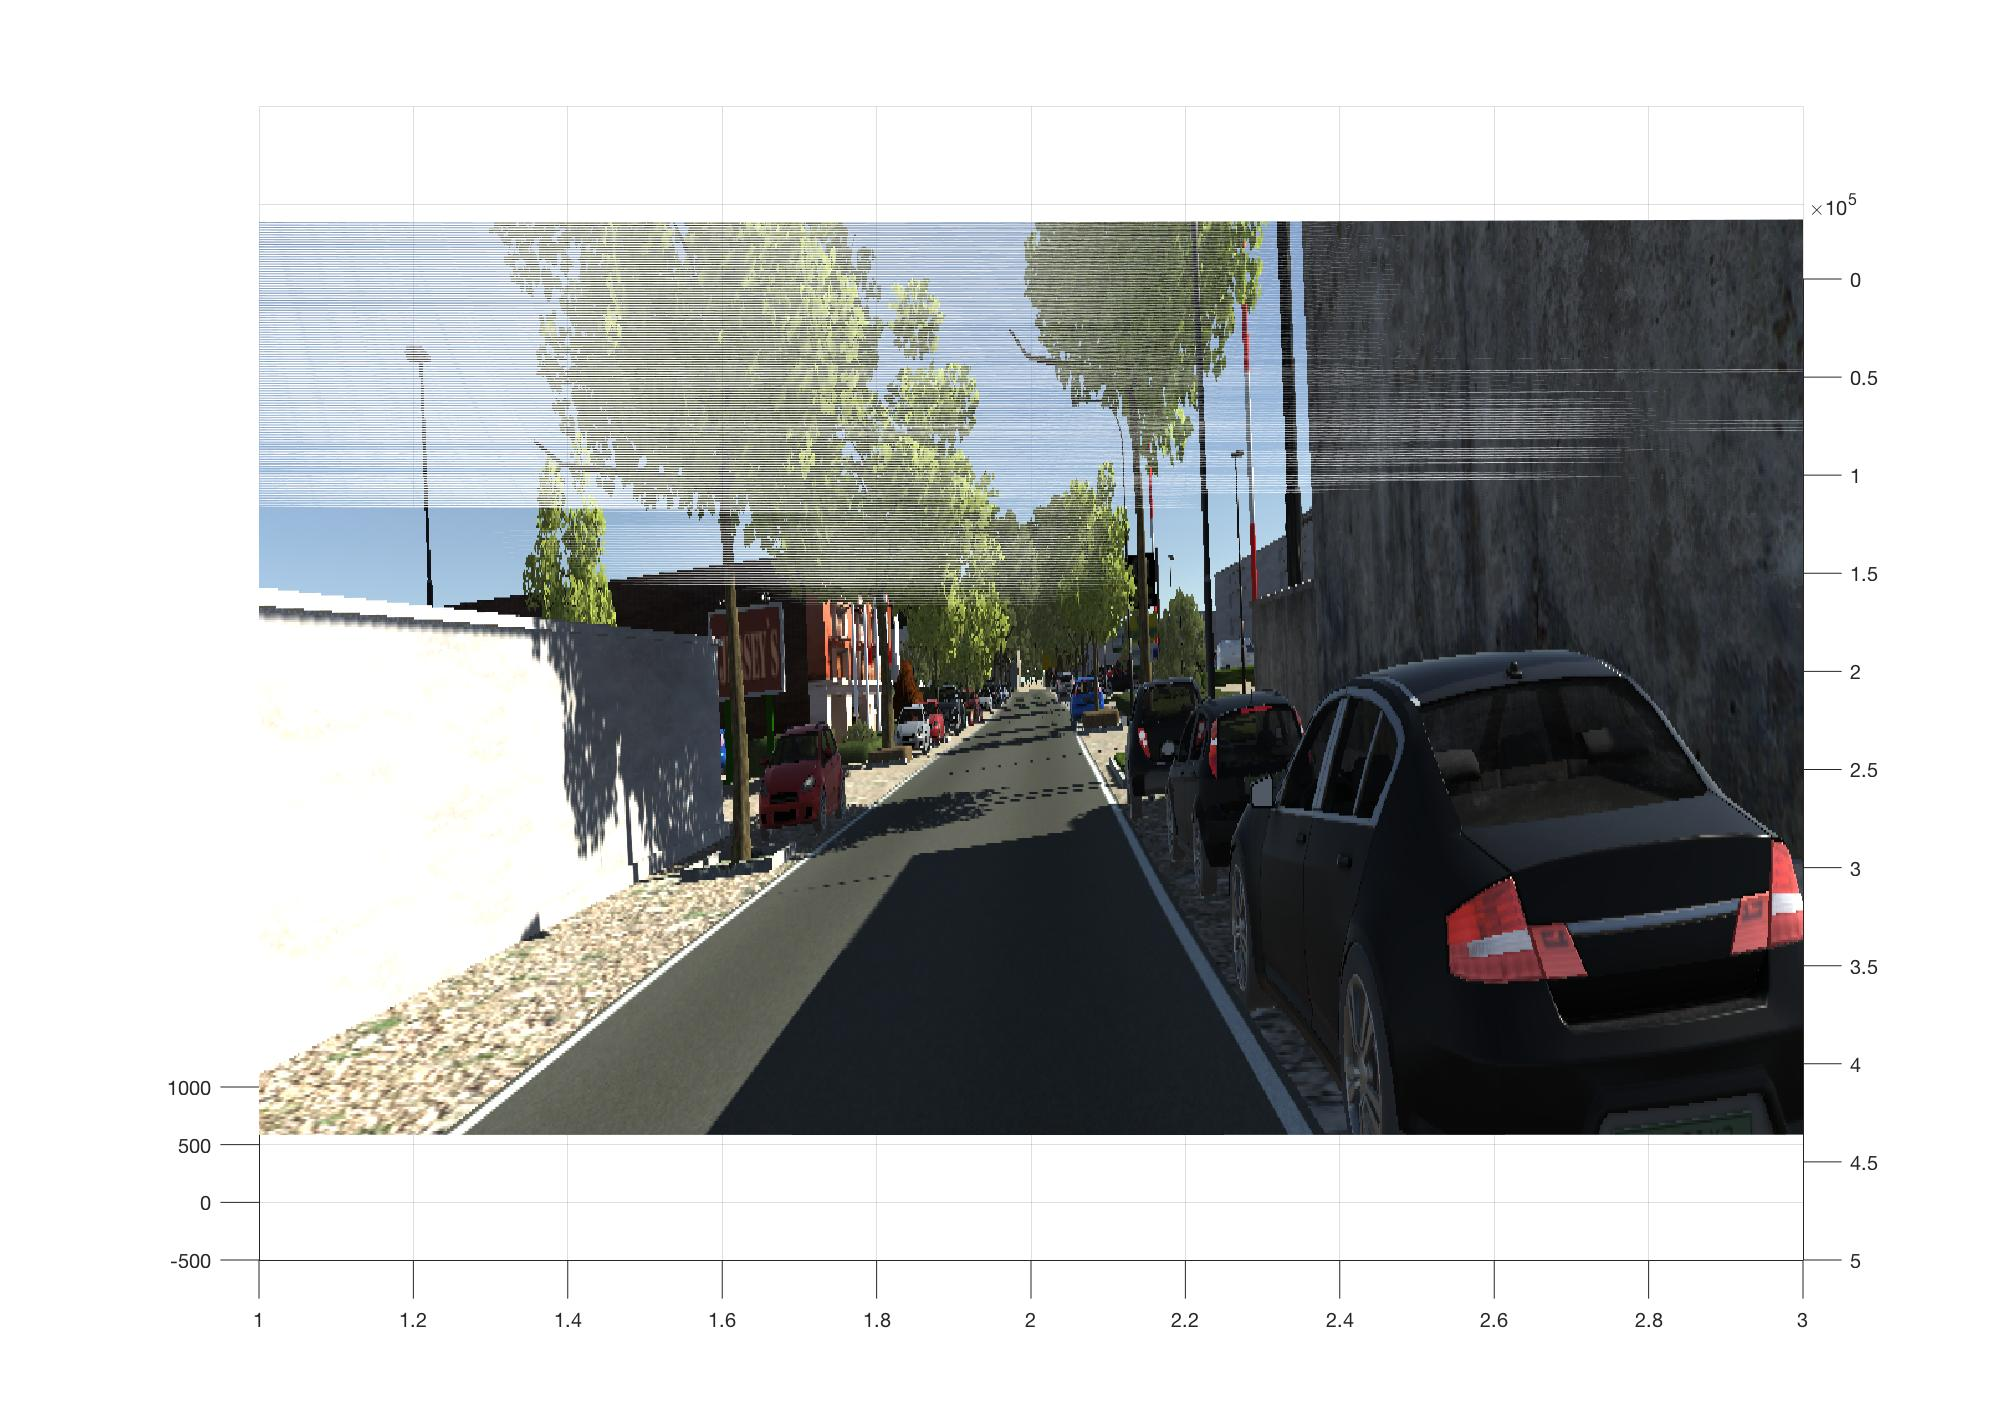
\includegraphics[width=\linewidth]{rgb-d-visualize.jpg}
    \caption{Visualized 3D scene}
  \end{subfigure}
\end{figure}

\clearpage
\item[Q4.]
\begin{enumerate}
\item Internal Camera Parameters Matrix 
\[
K =
  \begin{bmatrix}
    721.5 & 0 & 609.6 \\
    0 & 721.5 & 172.9 \\
    0 & 0 & 1
  \end{bmatrix}
\]
\end{enumerate}

\item Equation of the ground plane in camera coordinate system 
\[
  \vv{m}
  \begin{pmatrix}
  \begin{bmatrix}
    x \\
    y \\
    z 
  \end{bmatrix}
  - p
  \end{pmatrix}
  = 0
\]
where $\vv{m} = \begin{bmatrix}0,1,0\end{bmatrix}$ and $p = \begin{bmatrix}0,-1.7,0\end{bmatrix}$

\item To compute the 3D location of a 2D point $(x, y)$ given the camera matrix $K$ and disparity map; first we compute $Z = \frac{f . T}{x_{l} - x_{r}}$ where $f$ is the focal length, $T$ is the baseline value and $x_{l} - x_{r}$ is the from the disparity map. Now, since we now $(x, y)$, we can write $x = \frac{f . X}{Z} + p_{x}$ and $y = \frac{f . Y}{Z} + p_{y}$ where $p_{x}$ and $p_{y}$ are the principle points from $K$. We can rearrange the equations and solve for $X$ and $Y$. Hence, now we have our 3D location $(X, Y, Z)$ from a 2D point $(x, y)$.
\end{enumerate}

\item[Q5.] Extra Credit: I added the below code to Q2. in order to try to create a panorama!
\\ (P.S. I tried really hard to combine the 2 pieces but my application kept running out of memory :P)
\begin{lstlisting}[language=MATLAB]
# Read input images
img1 = cv2.imread('data/landscape_1.jpg')
img2 = cv2.imread('data/landscape_2.jpg')
img3 = cv2.imread('data/landscape_3.jpg')
img4 = cv2.imread('data/landscape_4.jpg')
img5 = cv2.imread('data/landscape_5.jpg')
img6 = cv2.imread('data/landscape_6.jpg')
img7 = cv2.imread('data/landscape_7.jpg')
img8 = cv2.imread('data/landscape_8.jpg')
img9 = cv2.imread('data/landscape_9.jpg')

# Use SIFT to find keypoints and compute homography matrix
# and Stitch the images together using homography matrix
M_1 =  compute_sift(img1, img2)
result_image_1 = stitch_images(img2, img1, M_1)

M_2 =  compute_sift(img3, img4)
result_image_2 = stitch_images(img4, img3, M_2)

M_3 =  compute_sift(img5, img6)
result_image_3 = stitch_images(img6, img5, M_3)

M_4 =  compute_sift(img7, img8)
result_image_4 = stitch_images(img8, img7, M_4)

M_5 = compute_sift(result_image_1, result_image_2)
result_image_5 = stitch_images(result_image_2, result_image_1, M_5)

M_6 = compute_sift(result_image_3, result_image_4)
result_image_6 = stitch_images(result_image_4, result_image_3, M_6)

M_7 = compute_sift(result_image_6, img9)
result_image_7 = stitch_images(img9, result_image_6, M_7)

*** OUTPUT ON THE NEXT PAGE ***
\end{lstlisting}

\newpage
\begin{figure}[t!]
  \centering
  \begin{subfigure}[b]{0.8\linewidth}
    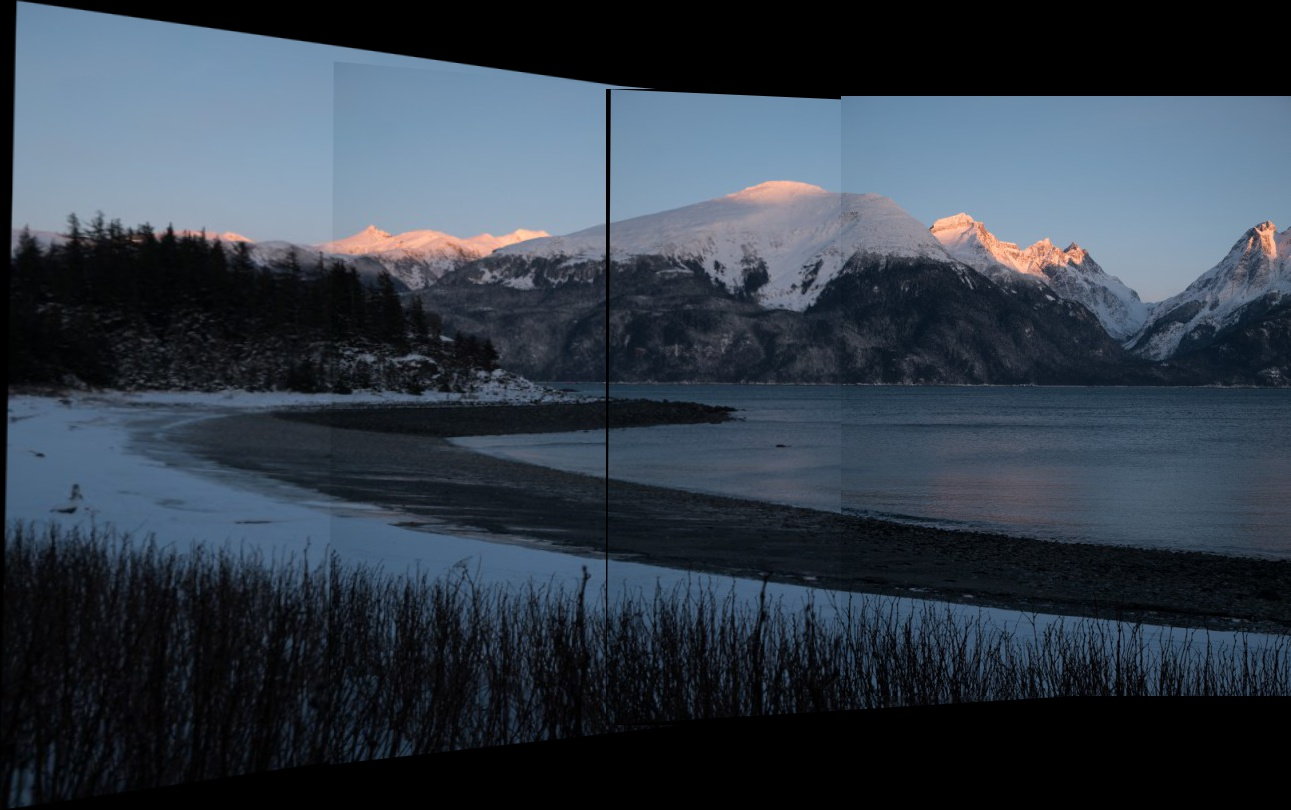
\includegraphics[width=\linewidth]{panorama_5.jpg}
    \caption{Panorama created from image landscapes 1 - 4}
  \end{subfigure}
  \begin{subfigure}[b]{0.8\linewidth}
    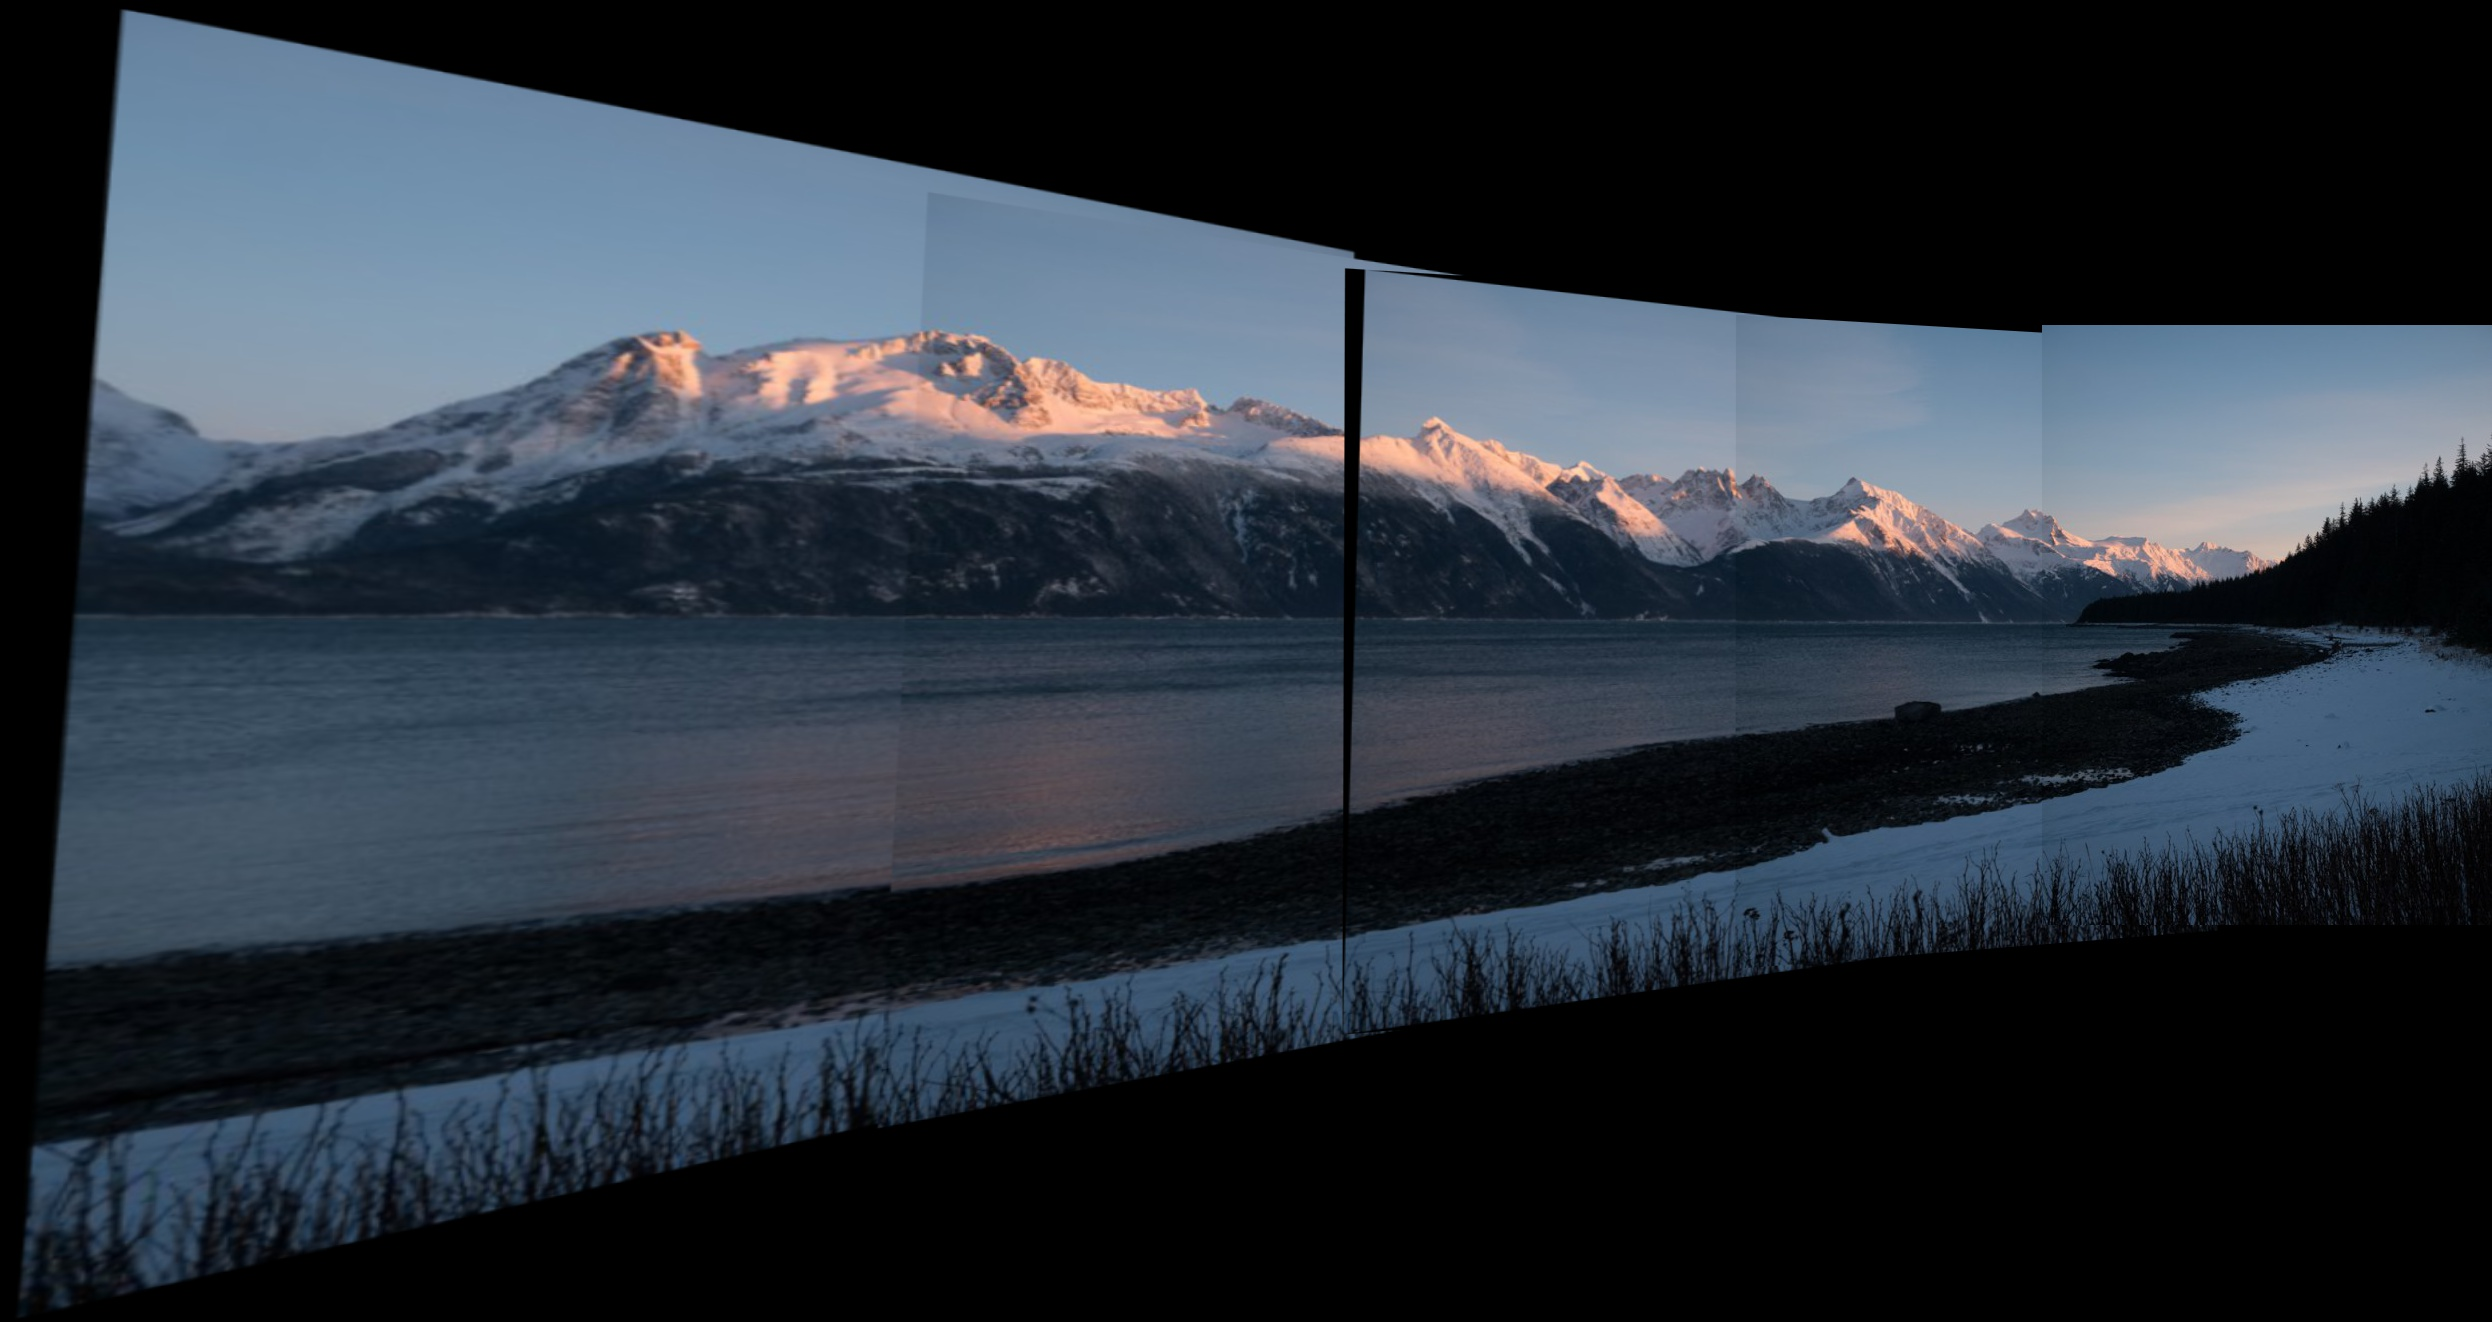
\includegraphics[width=\linewidth]{panorama_7.jpg}
    \caption{Panorama created from image landscapes 5 - 9}
  \end{subfigure}
\end{figure}

\clearpage
\end{description}
\end{document}
  
  



